\documentclass[runningheads]{llncs}
%
\let\subparagraph\paragraph % work around llncs/titlesec clash
\usepackage{titlesec}
\titlespacing*{\section}{0pt}{*1}{*1}
\titlespacing*{\subsection}{0pt}{*0.8}{*0.8}

\usepackage{enumitem}
\setlist[itemize]{topsep=0pt, partopsep=0pt, itemsep=0pt, parsep=0pt}
\setlist[enumerate]{topsep=0pt, partopsep=0pt, itemsep=0pt, parsep=0pt}

\setlength{\parskip}{0pt}
\setlength{\parindent}{1em}

\usepackage[T1]{fontenc}
\usepackage{graphicx}
\usepackage{booktabs}
\usepackage{amsmath,amssymb}
\usepackage{tikz}
\usetikzlibrary{shapes.geometric, arrows.meta, positioning}
\usepackage{algorithm}
\usepackage{algpseudocode}

\begin{document}
\flushbottom
\addtolength{\voffset}{-1.5cm}
\addtolength{\textheight}{1.5cm}

\title{Interpretable Stylometric Detection of Sentence-Level Author Switches in Multi-Author Documents}

\author{Tshephang Phuti-A-Nkutu Matlala}
\institute{University of Johannesburg, South Africa \\
\email{223004635@student.uj.ac.za}}

\titlerunning{Stylometric Detection of Author Switches}
\maketitle

\begin{abstract}
Detecting where one author's writing ends and another's begins within a single document, known as style change detection, is a
central problem in authorship analysis, with applications in forensic linguistics, academic integrity investigation, gift authorship
detection, and the moderation of anonymous online content. State of the art systems are increasingly transformer based and give little
insight into which linguistic properties signalled a change, which limits their use where an explanation is required. This paper
presents an interpretable, stylometrically grounded system for sentence level author switch detection, implemented from scratch in
Java. Each sentence is described by nine named stylometric scalars (length, frequent word ratio, punctuation density, digit and
uppercase ratio, average word length, mean TF-IDF, and a lexicon based emotion score) plus a hashed character trigram profile; a
sentence pair is represented by eleven features, namely the nine absolute standardised differences, the trigram cosine similarity,
and an overall distance. We motivate the hashed n gram profile by its fixed size and corpus independent cost, which keeps the approach
scalable to real world corpora. A decision tree, logistic regression, and a feed forward neural network are trained with class weighting
and a validation tuned decision threshold on the PAN 2026 multi-author writing style analysis data, and evaluated on a held out, document
disjoint test split of 259,653 sentence pairs. The three models reach F1 scores of 0.435 to 0.456 overall (balanced accuracy 0.66 to 0.67).
The result is strongly difficulty dependent: on easy pairs, where authorship changes coincide with topic changes, F1 is 0.85 to 0.87, whereas
on medium and hard pairs balanced accuracy is close to 0.50, i.e. the features carry almost no usable style signal once topic is controlled.
I have discussed what this shows about surface stylometry, and set out the investigations planned for the next phase.
\end{abstract}

\section{Introduction}

Authorship analysis is the branch of natural language processing concerned with identifying, verifying, or profiling the author of a text from
patterns in how it is written, rather than from explicit metadata about who wrote it \cite{bevendorff:2026a}. A central problem in this field
is style change detection: given a document that may contain contributions from more than one author, determine whether it is in fact
multi authored and, if so, identify the precise positions at which the writing style, and therefore we presumptive the author based on the changes \cite{zangerle2020overview}.

This is a substantially harder problem than single author attribution, which compares a disputed text against known writing samples from a small
set of candidates. Style change detection has no such reference: it must decide from the text alone whether an internal shift in style has
occurred using only the natural stylistic profile of each sentence segment \cite{ramnial2015authorship}. The difficulty is compounded when style
must be separated from topic level based, since if the shift is in subject matter it is easy to detect and often correlates with a change of author,
conflating topic segmentation with style analysis. The PAN shared task series at CLEF has progressively tightened this distinction: the task
overview describes an natural style change detection task in which all positions of writing style change must be found from 2025 onward this is
defined at the sentence level, with datasets organised into easy, medium, and hard difficulty levels that systematically reduce topical variety,
so that the hard condition forces systems to rely on style alone \cite{zangerle:2026,zangerle_2026_19068843}. This project is not sorely depended on
most accurate model as the competition is surely based on, but about learning which natural features are best to be used in this settings.

Several practical settings in which style change detection is useful specifically require an explanation and not just a decision. In forensic
linguistics, an expert witness must point to specific, defensible linguistic evidence, since a bare probability cannot meet that evidentiary
standard \cite{6722273}. In academic integrity work, the useful output for an investigator is not only the boundary but a stated reason,
for example a shift in sentence length, vocabulary richness, or punctuation habits. In collaborative writing, an explainable signal of who
wrote which section is more defensible than an opaque one when used to inform authorship credit, and in platform moderation, stylistic
evidence that a human can inspect is preferable to an opaque flag.

\textbf{(i) Existing work.} Existing stylometric systems, including Ochab et al.'s gradient boosted, frequency based
pipeline \cite{ochab2025styloch} and earlier PAN submissions, often rely on aggregate or document level statistics and
provide limited analysis of sentence level transitions. Recent transformer based and graph based systems have pushed
raw detection performance on PAN style benchmarks considerably higher than these classical stylometric
baselines \cite{chen2023writing,alsheddi2025team}, but almost universally is at the cost of attribution (a fine tuned
RoBERTa or DeBERTa classifier can flag a boundary with high confidence without indicating which stylistic dimension
drove that decision).

\textbf{(ii) However.} Neither line of work directly targets sentence level author switch detection with a
representation that is both transparent and pairwise in nature. Document or aggregate level stylometry, as in
Ochab et al.'s system is explainable but coarse, while transformer based detectors are finer grained but offer
no genuine attribution for a given boundary decision.

\textbf{(iii) Therefore.} This paper adopts an explicitly interpretable position for the sentence level author switch
problem specifically using transparent handcrafted stylometric representations that permit feature level interpretation
for every prediction rather than trying to match transformer level accuracy. The goal is to characterise how far a
fully interpretable, handcrafted stylometric system can go, and precisely where and why it fails.

\section{Problem Definition}

A document is treated as a sequence of sentences rather than as a single block of text, so that authorship boundaries
can be localised precisely rather than only detected at the document level. Formally, let a document $D$ consist of $n$
consecutive sentences $D = \{S_1, S_2, \ldots, S_n\}$. For every adjacent pair $(S_i, S_{i+1})$, the task is to predict
a binary boundary label
\[
y_i =
\begin{cases}
0 & \text{if } S_i \text{ and } S_{i+1} \text{ were written by the same author,} \\
1 & \text{if an author switch occurs between } S_i \text{ and } S_{i+1}.
\end{cases}
\]
The full sequence $\{y_1, \ldots, y_{n-1}\}$ determines the authorship structure of the entire document, namely whether
it is multi authored at all, how many authors contributed, and where each author's contiguous segments lie. Sentence
level detection is harder than the paragraph level formulation used in earlier PAN editions because each segment carries
only around fifteen to twenty words of stylistic evidence \cite{zangerle_2026_19068843}, and difficulty increases further
from easy, where author switches coincide with topic changes, through medium, to hard, where all sentences in a document
share one topic so that only style can be used \cite{zangerle2025overview}.

The natural evaluation metric is the F1 score over boundary predictions because the classes are heavily imbalanced.
Same author boundaries substantially outnumber genuine switches in realistic documents, so a majority class predictor
can reach high accuracy while identifying no switches at all. The imbalance is treated as a first class methodological
concern in Section 5 rather than an afterthought. This research is organised around four questions.
\textbf{RQ1}: How well can a small, fully named set of stylometric features detect sentence level author switches, and
how does performance change from the easy to the hard condition?
\textbf{RQ2}: Do a decision tree, logistic regression, and a neural network models differ meaningfully on this
representation, and what does that imply about the shape of the decision boundary?
\textbf{RQ3}: How does class imbalance, class weighting, and decision threshold tuning affect the precision recall
trade off?
\textbf{RQ4}: Which features from the trained models carry the signal, and what is the gap to transformer based systems
suggest about which parts of the problem are recoverable from surface statistics?

\section{Related Work}

Style change detection has been studied continuously within the PAN shared task series since 2016 moving from document
level single versus multi author classification to paragraph level boundary detection to the current sentence level
formulation \cite{bevendorff2021overview,zangerle_2026_19068843}. A recurring methodological concern across editions
has been the confound between topic and style. Early datasets allowed systems to succeed largely by detecting topic
shifts in which the 2023 through 2026 editions deliberately control for through the easy, medium, and hard difficulty
stratification \cite{zangerle2025overview}. The task overview paper for the lab as a whole situates style change
detection alongside the other PAN 2026 tasks and motivates the shared evaluation infrastructure used across
them \cite{zangerle:2026}. The 2026 edition additionally moves to a fan fiction derived dataset specifically to obtain
longer, topic based, and coherent short pieces of writing while retaining precise control over authorship boundaries \cite{bevendorff:2026b}.

Stylometric authorship analysis comes before modern natural language processing. Classic case studies, such as the
disputed Federalist Papers established that function word and punctuation statistics can carry a detectable, largely
unconscious authorial signature, and Jockers and Witten later gave a systematic comparison of machine learning methods
for this kind of attribution \cite{10.1093/llc/fqq001}. Ramnial et al.\ reframed attribution as pairwise binary
verification in which two adjacent segments are compared and a boundary is inferred if they differ enough
stylistically \cite{ramnial2015authorship}. This is the representation adopted by the project. Singh et al.\ combined
character n-grams, part of speech tag, function word frequencies, and vocabulary richness statistics into pairwise
absolute feature differences and classified with logistic regression and reached an F1 score of 0.657 at the paragraph
level on PAN 2021 data \cite{singh2021writing}. This remains the closest direct methodological precedent for the
project system just extended to the sentence level with a broader feature set. Rios Toledo et al.\ found that higher
order character n-grams and part of speech tag sequences outperform unigrams and are comparatively robust to topic shift
in literary text \cite{rios2022detection}. Hossain et al.\ combined stylometric features with shallow neural classifiers
for author attribution. Alshamasi and Menai applied ensemble k-means clustering directly to stylistic feature vectors,
reaching an F1 score of approximately 0.49 at the sentence level without any supervision \cite{alshamasi2022ensemble},
which is a useful unsupervised reference point and motivates including density based clustering, such as HDBSCAN as a
comparison method in future work. Zamir et al.\ argue explicitly against stripping punctuation and stop words during
preprocessing for this task, since they carry authorial signal that content word only pipelines would
discard \cite{zamir2024stylometry}, a design choice retained here. Most directly relevant to the present system's
positioning, Ochab et al.\ build a modular, non neural stylometric pipeline in which linguistic annotation feeds several
thousand frequency features into a gradient boosted classifier presented explicitly as an inexpensive and explainable
alternative to transformer based detectors, and reported as competitive on a related PAN authorship task \cite{ochab2025styloch}.
The overview of PAN 2025 similarly notes that at least one competitive team combined stylometric features with sentence
embeddings feeding a gradient boosting classifier \cite{zangerle2025overview} indicating that gradient boosted stylometric
pipelines remain a live and effective design choice even as the field's centre of mass moves toward transformers.

Neural methods report the strongest raw performance on current PAN benchmarks. Chen et al.\ proposed a contrastive
learning writing style embedding for multi author analysis \cite{chen2023writing}. Alsheddi and Menai modelled each
sentence as a graph node and used graph convolutional networks to propagate authorship consistency signal between
sentences for PAN 2025 \cite{alsheddi2025team}. Lin et al.\ fine tuned deep architectures for the same task family,
and a related supervised contrastive DeBERTa variant further improved detection through contrastive pretraining
objectives specific to style change. At PAN 2025, Rohra et al.\ fine tuned RoBERTa directly on the sentence pair
formulation of the task \cite{rohra2025sentence}, and the ARC-NLP team reframed paragraph level style change
detection at PAN 2023 as a natural language inference problem, learning whether two consecutive segments entail
the same author or not \cite{kucukkaya2023arc}. Most strikingly, a PAN 2025 submission by the team named better call claude
showed that a large language model used largely zero shot, exploiting sequential and contextual cues across a document,
was competitive with purpose trained classifiers, while explicitly flagging that this success may partly reflect exploitation
of document macrostructure rather than isolation of intrinsic stylistic signal, and recommending that future task
editions control for this by testing under randomised sentence order \cite{schmidt2025team}. This observation is directly relevant to the present work's stylometric, order independent, pairwise design, which cannot exploit that kind of contextual shortcut and should therefore be measuring something closer to genuine style discrimination.

Across both families of prior work, The systems either optimise purely for benchmark performance without exposing which
linguistic dimensions drove a given prediction or they use comparatively narrow, fixed stylometric feature sets without
a systematic per group importance analysis under the sentence level, difficulty stratified conditions introduced from
PAN 2025 onward. The gap this project targets is a stylometric pipeline broad and carefully justified enough to be a
meaningful comparison point, instrumented specifically so that every prediction is attributable to named features, and
evaluated with a methodology that avoids the specific pitfalls identified in review of the earlier exploratory version
of this system.

\section{Proposed System}

\begin{figure}[t]
\centering
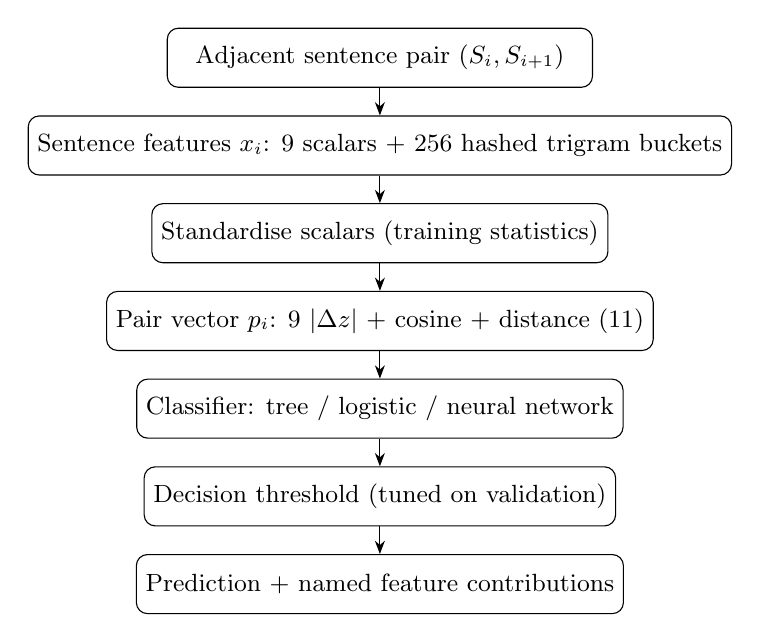
\begin{tikzpicture}[
  node distance=0.35cm,
  box/.style={rectangle, draw, rounded corners, minimum width=5.4cm, minimum height=0.75cm, align=center, font=\small},
  arr/.style={-Stealth}
]
\node[box] (pair) {Adjacent sentence pair $(S_i, S_{i+1})$};
\node[box, below=of pair] (feat) {Sentence features $x_i$: 9 scalars + 256 hashed trigram buckets};
\node[box, below=of feat] (z) {Standardise scalars (training statistics)};
\node[box, below=of z] (pv) {Pair vector $p_i$: 9 $|\Delta z|$ + cosine + distance (11)};
\node[box, below=of pv] (clf) {Classifier: tree / logistic / neural network};
\node[box, below=of clf] (thr) {Decision threshold (tuned on validation)};
\node[box, below=of thr] (pred) {Prediction + named feature contributions};
\foreach \a/\b in {pair/feat, feat/z, z/pv, pv/clf, clf/thr, thr/pred}
  \draw[arr] (\a) -- (\b);
\end{tikzpicture}
\caption{Overview of the sentence level author switch detection pipeline.}
\label{fig:pipeline}
\end{figure}

\subsection{Implementation}
The system is written in Java 25 (Temurin) and deliberately uses no external machine learning library: the feature extractor, the decision tree, logistic regression, and the neural network are all implemented from scratch, so every step from raw text to prediction can be inspected. The same \texttt{data}, \texttt{features}, and \texttt{models} packages are used by two front ends: a command line trainer (\texttt{Main.java}, launched by \texttt{build.sh} or \texttt{build.bat}, needing only \texttt{javac} and \texttt{java}) and a Spring Boot web application with Inspect, Explore, Train, Predict, and Results pages. Training, model persistence, and prediction share one code path, and trained models and metrics are written to the same files the web application reads, so a reported result corresponds to the exact artefact used for prediction. As a consistency check, the memory efficient feature matrix builder recomputes 200 pairs the original way and confirms identical output.

\subsection{Sentence features}
Fig.~\ref{fig:pipeline} summarises the pipeline. Following Zamir et al.\ \cite{zamir2024stylometry}, punctuation, stop words, and capitalisation are retained rather than stripped. Each sentence $S_i$ is mapped by $f$ to a vector
\begin{equation}
x_i = f(S_i) = [\,x_i^{(1)},\ldots,x_i^{(9)},\; h_i\,],
\label{eq:sentvec}
\end{equation}
where $x_i^{(1..9)}$ are the named scalar features of Table~\ref{tab:features} and $h_i\in\mathbb{R}^{256}$ is a hashed character trigram profile described below. The scalars are z-score standardised using means and standard deviations fitted on the training sentences only.

\begin{table}[t]
\centering
\caption{Stylometric features used in the trained models. Index refers to the pair vector position used in Section~\ref{sec:results}.}
\label{tab:features}
\begin{tabular}{p{0.6cm}p{3.1cm}p{3.6cm}p{3.6cm}}
\toprule
\textbf{Idx} & \textbf{Feature} & \textbf{Definition} & \textbf{Motivation} \\
\midrule
0 & Word length & $\log(1+\#\text{words})$ & Fluency, segment length \cite{10.1093/llc/fqq001} \\
1 & Character length & $\log(1+\#\text{chars})$ & As above \\
2 & Frequent word ratio & share of tokens in the 10,000 most common English words & Function word like habit \cite{6722273} \\
3 & Punctuation density & count of \texttt{! ; , . ? ' "} per character & Unconscious habit \cite{zamir2024stylometry} \\
4 & Digit ratio & digits per character & Formatting habit \\
5 & Uppercase ratio & uppercase letters per character & Capitalisation habit \\
6 & Average word length & letters per word & Vocabulary register \\
7 & Mean TF-IDF & mean TF-IDF of tokens, IDF from training sentences & Vocabulary rarity \\
8 & Emotion score & NRC lexicon \cite{mohammad2013crowdsourcing}, length normalised & Affective tone \\
\bottomrule
\end{tabular}
\end{table}

Two points should be noted about Table~\ref{tab:features}. First, feature 2 uses a list of frequent words (Google 10,000 English) rather than a curated closed class function word list, so it only approximates the classical function word signal. Second, part of speech, readability, type token ratio, and positional feature groups are not implemented in the trained system, and are therefore left to future work. The Explore page shows a sentence position value for each pair, but it is not part of the trained vector.

\subsection{Hashed character n grams and scalability}
Rios Toledo et al.\ \cite{rios2022detection} and Ochab et al.\ \cite{ochab2025styloch} show that character n grams are a strong, topic robust authorship signal, but the usual formulation builds an explicit n gram vocabulary. Ochab et al.\ feed several thousand frequency features to a gradient boosted classifier. That design scales badly to real world corpora: the vocabulary of character and word n grams grows with corpus size and with n, every new document may require extending or refitting the feature space, and the feature matrix grows with the vocabulary, so both the time to generate features and the memory needed to hold them rise with data volume. For a deployed tool that must process large, previously unseen collections, this becomes the dominant cost.

The project instead uses the hashing trick. Each character trigram of a sentence is mapped to one of $B=256$ buckets by a hash of the trigram, counts are normalised by the number of trigrams, and the result is $h_i$. This has three properties relevant to scale. (i) The vector length is fixed at 256 regardless of corpus size, so memory per sentence is constant. (ii) No vocabulary pass or dictionary is needed, so unseen words and trigrams are handled automatically and features can be computed in a single streaming pass, in time linear in sentence length. (iii) Sentences are processed independently, so extraction parallelises trivially. The costs are hash collisions, which merge unrelated trigrams into one bucket, and the loss of bucket level interpretability, since a bucket is not a readable unit. The profile is therefore exposed to the model only as a single, readable quantity: the cosine similarity between $h_i$ and $h_{i+1}$, i.e.\ ``how similar are the character level profiles of the two sentences''. This compression reduces the pair vector from 267 columns (9 + 2 + 256 bucket differences) to 11, roughly a 24 fold reduction in matrix width, and all reported results use the 11 column form; the 267 column form is implemented but was not used. The project has not benchmarked wall clock extraction time against an explicit n gram vocabulary, so the scalability claim here is structural rather than measured; doing so is listed under future work. The mean TF-IDF feature is the one remaining component that needs a corpus level pass, to build document frequencies.

\subsection{Pairwise representation and classifiers}
For each boundary $(S_i,S_{i+1})$ the pair vector $p_i = g(x_i,x_{i+1})\in\mathbb{R}^{11}$ is
\begin{equation}
\begin{split}
p_i &= \big[\,|z_i^{(1)}-z_{i+1}^{(1)}|,\ldots,|z_i^{(9)}-z_{i+1}^{(9)}|,\ \cos(h_i,h_{i+1}),\ d_i\,\big],\\
d_i &= \sqrt{\tfrac{1}{9}\textstyle\sum_{k=1}^{9}\big(z_i^{(k)}-z_{i+1}^{(k)}\big)^2},
\end{split}
\label{eq:pairvec}
\end{equation}
where $z$ denotes the standardised scalar. Only the absolute difference form \cite{ramnial2015authorship,singh2021writing} is implemented; the concatenation and union forms are not. A classifier then maps $p_i$ to a label, $\hat{y}_i = C(p_i)$. Three from scratch classifiers are compared:
\begin{itemize}
\item \textbf{Decision tree}: Gini impurity, maximum depth 5, minimum 20 samples to split and 5 per leaf, class weighted, threshold fixed at 0.5. Its rules are directly readable.
\item \textbf{Logistic regression}: batch gradient descent, 10,000 iterations, learning rate 0.6, class weighted. Its 11 weights are directly readable.
\item \textbf{Neural network}: 11--128--64--32--16--8--1, ReLU hidden layers, sigmoid output, plain mini batch stochastic gradient descent (learning rate 0.001, batch 64, no momentum or adaptive step), L2 penalty 0.01, dropout 0.2, feature clipping to $[-5,5]$, class weighted loss, at most 60 epochs with early stopping on validation loss (patience 8).
\end{itemize}
A random forest is also implemented in the code base but was not run for this paper. Gradient boosted models and scikit-learn baselines were not built, so the from scratch models are the whole comparison.

\begin{algorithm}[t]
\caption{End-to-end training and prediction pipeline}
\label{alg:pipeline}
\begin{algorithmic}[1]
\Require Training pairs $\{(S_i,S_{i+1},y_i)\}$, validation pairs, test pairs
\State Fit IDF table and scalar means/standard deviations on training sentences
\For{each pair}
    \State $x_i \gets f(S_i)$, $x_{i+1}\gets f(S_{i+1})$ \Comment{Eq.~\eqref{eq:sentvec}}
    \State $p_i \gets g(x_i,x_{i+1})$ \Comment{Eq.~\eqref{eq:pairvec}}
\EndFor
\State Train $C$ on training pairs with inverse frequency class weights
\State Choose threshold $\tau$ maximising F1 on the validation half
\State Report metrics on the held out test half using $\tau$
\State \Return model, $\tau$, metrics
\end{algorithmic}
\end{algorithm}

\section{Evaluation Methodology}
\label{sec:eval}

\textbf{Data.} The project uses the PAN 2026 multi-author writing style analysis data \cite{zangerle_2026_19068843}, fanfiction derived and split into easy, medium, and hard difficulty. Table~\ref{tab:data} gives the training set statistics. The switch rate differs sharply by difficulty (30.5\%, 4.4\%, 20.9\%), and overall 14.3\% of the 2,439,074 training pairs are switches.

\begin{table}[t]
\centering
\caption{Training set statistics per difficulty (10,500 problems each).}
\label{tab:data}
\begin{tabular}{lrrrr}
\toprule
\textbf{Difficulty} & \textbf{Sentences} & \textbf{Pairs} & \textbf{Switches} & \textbf{Switch rate} \\
\midrule
Easy   & 560,304   & 549,804   & 167,801 & 30.52\% \\
Medium & 1,309,824 & 1,299,324 & 56,631  & 4.36\% \\
Hard   & 600,446   & 589,946   & 123,564 & 20.94\% \\
\midrule
All    & 2,470,574 & 2,439,074 & 347,996 & 14.27\% \\
\bottomrule
\end{tabular}
\end{table}

\textbf{Splits.} Training uses all three difficulties combined. Because the official test labels are not available to us, the official validation set is divided into two halves by problem, using a fixed seed shuffle, so no document contributes to both halves. The first half (264,150 pairs, 14.51\% switches) is used for early stopping and threshold selection; the second half (259,653 pairs, 14.06\% switches) is the held out \emph{test} split, touched only once for final numbers. All 2,439,074 training pairs are used. Training documents are disjoint from both, so no document specific style leaks across splits. A single fixed, document disjoint split is therefore used instead of grouped cross validation, which is cheaper but gives no variance estimate.

\textbf{Imbalance handling.} Loss is weighted by inverse class frequency (weights 0.583 for same author and 3.505 for switch). For the logistic regression and neural network the decision threshold is swept on the validation half to maximise F1; the tree keeps 0.5. SMOTE \cite{chawla2002smote} and resampling were not used.

\textbf{Metrics.} Accuracy, precision, recall, F1 for the switch class, and balanced accuracy, overall and per difficulty. Accuracy is always shown against the majority class baseline, because a model that never predicts a switch already scores 85.9\% on the test split.

\section{Results}
\label{sec:results}

All three models were trained on the complete training set of 2,439,074 pairs. Table~\ref{tab:overall} reports the held out test results. The models are close: F1 ranges from 0.435 (tree) to 0.456 (logistic regression), and balanced accuracy from 0.661 to 0.669. Logistic regression is best on F1 and balanced accuracy, the neural network has the highest precision (0.562) and accuracy (0.871), and the tree has the highest recall (0.410). The neural network is not better than the linear model. Logistic regression converged: its training loss reaches 0.58691 by about iteration 8,400 and the last 5,000 iterations change it by roughly $3\times10^{-5}$, so more iterations would not help. This points to a limit in the 11 features rather than in model capacity or training length.

\begin{table}[t]
\centering
\caption{Held out test results (259,653 pairs), all difficulties, models trained on all 2,439,074 training pairs. Majority baseline accuracy is 0.8594.}
\label{tab:overall}
\begin{tabular}{lccccccc}
\toprule
\textbf{Model} & \textbf{Thr.} & \textbf{Acc.} & \textbf{Prec.} & \textbf{Rec.} & \textbf{F1} & \textbf{Bal.\ Acc.} \\
\midrule
Decision tree       & 0.50 & 0.8499 & 0.4622 & 0.4104 & 0.4348 & 0.6661 \\
Logistic regression & 0.68 & 0.8686 & 0.5457 & 0.3915 & 0.4559 & 0.6691 \\
Neural network      & 0.66 & 0.8708 & 0.5620 & 0.3682 & 0.4449 & 0.6606 \\
\bottomrule
\end{tabular}
\end{table}

\textbf{Reading the metrics.} For the tree, of 32,420 pairs flagged as switches 14,986 are real (precision 0.462), and of 36,517 real switches 14,986 are found (recall 0.410). Accuracy is not informative here: a classifier that never predicts a switch scores 0.8594, and only logistic regression (0.8686) and the neural network (0.8708) exceed it, and only marginally. The tree is below it (0.8499) because class weighting makes it over predict switches at a fixed threshold of 0.5.

\textbf{Threshold tuning matters (RQ3).} With the default 0.5 threshold, logistic regression on the validation half scored accuracy 0.725, precision 0.284, recall 0.589, F1 0.383. Tuning to 0.68 raised validation F1 to 0.472 and accuracy to 0.868, and test F1 was 0.456. Class weighting pushes the models to over predict switches, so a higher threshold recovers precision at the cost of recall. The tree keeps 0.5, so its accuracy and precision are not directly comparable with the other two models.

\textbf{Results depend almost entirely on difficulty (RQ1).} Table~\ref{tab:diff} shows the breakdown. On easy pairs, where author changes coincide with topic changes, all models are strong (F1 0.848 to 0.872, balanced accuracy 0.873 to 0.897), with very high precision for the linear and neural models (0.96). On medium and hard pairs balanced accuracy is between 0.499 and 0.515, indistinguishable from chance. The overall F1 of about 0.45 is therefore an average of a good easy result and a near chance result on the 78\% of test pairs that are medium or hard (139,254 and 63,714 pairs against 56,685 easy).

\begin{table}[t]
\centering
\caption{Held out test F1 / balanced accuracy per difficulty. The last row is the F1 of a trivial classifier that always predicts ``switch'', computed from the class counts.}
\label{tab:diff}
\begin{tabular}{lccc}
\toprule
\textbf{Model} & \textbf{Easy} & \textbf{Medium} & \textbf{Hard} \\
\midrule
Decision tree       & 0.872 / 0.897 & 0.067 / 0.503 & 0.057 / 0.502 \\
Logistic regression & 0.869 / 0.890 & 0.078 / 0.515 & 0.040 / 0.503 \\
Neural network      & 0.848 / 0.873 & 0.058 / 0.503 & 0.027 / 0.499 \\
\midrule
Always ``switch'' (F1 only) & 0.458 & 0.085 & 0.349 \\
\bottomrule
\end{tabular}
\end{table}

An important sanity check is the last row. On medium and hard pairs, all three models score \emph{below} the F1 of a classifier that flags every boundary as a switch (0.085 and 0.349). The models were tuned for the mixed, overall distribution, and on hard pairs recall collapses to 1.4 to 3.2\%. On topic controlled data the models have not learned a usable switch signal, and any deployment on such data would need a difficulty specific threshold and, more importantly, better features.

\textbf{What the models used.} The trained models are readable. The tree's root splits on the character length difference (feature 1), then on the average word length difference (feature 6), and the trigram cosine similarity (feature 9) appears at nearly every level. Only five of the eleven features are used at all (length in words and characters, punctuation density, average word length, and the trigram cosine); depth 5 allows at most 15 splits, and several splits end in two leaves of the same class, so the tree is effectively smaller than its shape suggests. A single depth limited tree is also a fragile guide to feature importance, since a different training sample can select different features. The logistic regression uses all 11 features and gives the largest weight to the trigram cosine (feature 9, $-4.71$, so more similar profiles mean fewer switches), followed by the character length difference (feature 1, $+0.99$) and the overall distance (feature 10, $+0.72$); the frequent word ratio and punctuation density differences receive weights near zero. Weights are not directly comparable across features, since the cosine is not standardised. Both models thus agree that the signal is dominated by \emph{how different the two sentences are in length and character level profile}. These are exactly the properties that also change when the topic or scene changes, which is consistent with the strong easy result and the collapse on medium and hard. This reading comes from model structure and is not a controlled ablation.

\textbf{Limitations.} (i) A single split, no confidence intervals, and a test split drawn from the official validation set. (ii) Only 11 pair features; the 256 bucket differences were not used. (iii) No hyperparameter search was reported for the final table beyond the fixed settings above; in particular the tree depth is fixed at 5. (iv) Each boundary is classified independently, discarding document context. (v) No comparison with transformer systems on the same split has been run. (vi) Some training sentences are extreme outliers (the maximum standardised average word length difference is 589 in training but 34 in validation), which particularly affects the linear model.

\section{Discussion}

The results give a clear answer to the guiding question of how far a fully interpretable, handcrafted stylometric system can go: on topic correlated switches it goes a long way (F1 about 0.87), and on topic controlled switches it currently does not go beyond chance. This matches the motivation behind the easy, medium, and hard design \cite{zangerle2025overview}: a system can look adequate overall while relying largely on topic. The easy result should therefore not be read as evidence of stylistic discrimination, and the overall F1 should not be quoted without the per difficulty breakdown.

The three models being nearly tied suggests that with these features the limiting factor is information, not model class. A depth 5 tree, a linear model, and a five hidden layer network reach almost the same balanced accuracy, and extra training does not help. This is a useful negative result: it argues against spending effort on larger models before richer, style specific features are added. Whether tree ensembles would help, as the gradient boosted pipelines in the literature \cite{ochab2025styloch,zangerle2025overview} suggest, remains untested here.

The reported medium and hard failure has a second cause worth stating. The nine scalars are largely surface statistics (length, letter case, punctuation rate), which vary between sentences of the same author at least as much as between authors, particularly in fiction where sentence length depends on narrative content. Function word profiles, syntactic patterns, and richer character n gram information are the features the literature reports as topic robust \cite{singh2021writing,rios2022detection}, and most of them are absent from the trained vector: the 256 trigram buckets are collapsed to one cosine, and part of speech and function word features are not implemented. The hashing design gives a way to restore this information without the vocabulary cost discussed earlier, by feeding bucket level differences, or several hashed n gram orders, to the models.

Interpretability, cost, deployment, and auditability remain the reasons to pursue this approach, and the Java implementation supports them: no GPU, no external libraries, one code path from training to prediction, and readable models. But the results show that interpretability alone is not sufficient. A readable model that is at chance on hard pairs offers no defensible evidence to a forensic examiner. The value of the current system is therefore mainly as a transparent baseline that quantifies how much of the task is recoverable from cheap surface statistics.

\section{Conclusion and Future Work}

This paper presented an interpretable Java based system for sentence level author switch detection, with nine named stylometric features, a hashed character trigram profile motivated by scalability, an eleven feature pairwise representation, and three from scratch classifiers evaluated on the PAN 2026 data. On a held out, document disjoint test split, logistic regression, a neural network, and a decision tree reached F1 of 0.456, 0.445, and 0.435. Performance is driven by the easy condition (F1 up to 0.872); on medium and hard pairs balanced accuracy is about 0.50 and F1 is below that of a trivial always switch classifier.

The investigations planned next follow directly from these findings:
\begin{itemize}
\item \textbf{Feature ablation and importance.} Leave one feature out and single feature runs, and permutation importance, to replace the structure based reading above with measured contributions.
\item \textbf{Restoring n gram information.} Use the full 267 column vector (256 bucket differences), several hashed n gram orders (character 2 to 5, word bigrams), and larger bucket counts, and measure both gain and cost; then benchmark feature generation time and memory against an explicit n gram vocabulary on progressively larger corpora to verify the scalability argument with measurements.
\item \textbf{Topic robust features.} Implement part of speech tag n grams, a closed class function word list, readability measures, and vocabulary richness, which are described in the literature but absent from the trained vector.
\item \textbf{Robustness and model tuning.} Clip or robustly scale outlier feature values (especially for logistic regression); tune and prune the tree depth beyond 5; and stabilise feature importance across repeated runs, since a single shallow tree selects only a few features.
\item \textbf{Difficulty aware decisions.} Per difficulty thresholds, or a difficulty estimator, since one threshold cannot suit switch rates of 30.5\%, 4.4\%, and 20.9\%.
\item \textbf{Stronger models and evaluation.} Random forest (already implemented) and gradient boosted trees; repeated splits or document grouped cross validation with confidence intervals; and the official test data when available.
\item \textbf{Estimating the number of authors.} Detected switches divide a document into segments, and the number of segments is an upper bound on the number of authors. How tight that bound is depends on the accuracy of the switch detector, since missed switches undercount segments and false switches inflate them. To estimate the number of authors, clustering algorithms such as k-means, hierarchical clustering, and Gaussian mixtures will be trained on the stylometric vectors of the segments, with the number of clusters limited to the number of segments and chosen by an internal criterion such as the silhouette score. This is only meaningful once the detector is better than chance on medium and hard pairs.
\item \textbf{Context.} A sliding window over several sentences, and a comparison with the transformer based systems surveyed in Section~3 on the same split, to quantify the interpretability and accuracy trade off rather than assert it.
\end{itemize}

Rather than replacing transformer based methods, this work asks whether interpretable stylometric models can become competitive enough for high stakes applications where explanation is required. The present evidence says that, with surface features alone, they cannot yet do so on topic controlled data, and it identifies where to look next.

%
% ---- Bibliography ----
%
\bibliographystyle{splncs04}
\bibliography{references}

\end{document}